\documentclass{ximera}

%\usepackage{todonotes}

\newcommand{\todo}{}

\usepackage{esint} % for \oiint
\ifxake%%https://math.meta.stackexchange.com/questions/9973/how-do-you-render-a-closed-surface-double-integral
\renewcommand{\oiint}{{\large\bigcirc}\kern-1.56em\iint}
\fi


\graphicspath{
  {./}
  {ximeraTutorial/}
  {basicPhilosophy/}
  {functionsOfSeveralVariables/}
  {normalVectors/}
  {lagrangeMultipliers/}
  {vectorFields/}
  {greensTheorem/}
  {shapeOfThingsToCome/}
  {dotProducts/}
  {partialDerivativesAndTheGradientVector/}
  {../productAndQuotientRules/exercises/}
  {../normalVectors/exercisesParametricPlots/}
  {../continuityOfFunctionsOfSeveralVariables/exercises/}
  {../partialDerivativesAndTheGradientVector/exercises/}
  {../directionalDerivativeAndChainRule/exercises/}
  {../commonCoordinates/exercisesCylindricalCoordinates/}
  {../commonCoordinates/exercisesSphericalCoordinates/}
  {../greensTheorem/exercisesCurlAndLineIntegrals/}
  {../greensTheorem/exercisesDivergenceAndLineIntegrals/}
  {../shapeOfThingsToCome/exercisesDivergenceTheorem/}
  {../greensTheorem/}
  {../shapeOfThingsToCome/}
  {../separableDifferentialEquations/exercises/}
  {vectorFields/}
}

\newcommand{\mooculus}{\textsf{\textbf{MOOC}\textnormal{\textsf{ULUS}}}}

\usepackage{tkz-euclide}
\usepackage{tikz}
\usepackage{tikz-cd}
\usetikzlibrary{arrows}
\tikzset{>=stealth,commutative diagrams/.cd,
  arrow style=tikz,diagrams={>=stealth}} %% cool arrow head
\tikzset{shorten <>/.style={ shorten >=#1, shorten <=#1 } } %% allows shorter vectors

\usetikzlibrary{backgrounds} %% for boxes around graphs
\usetikzlibrary{shapes,positioning}  %% Clouds and stars
\usetikzlibrary{matrix} %% for matrix
\usepgfplotslibrary{polar} %% for polar plots
\usepgfplotslibrary{fillbetween} %% to shade area between curves in TikZ
%\usetkzobj{all}
\usepackage[makeroom]{cancel} %% for strike outs
%\usepackage{mathtools} %% for pretty underbrace % Breaks Ximera
%\usepackage{multicol}
\usepackage{pgffor} %% required for integral for loops



%% http://tex.stackexchange.com/questions/66490/drawing-a-tikz-arc-specifying-the-center
%% Draws beach ball
\tikzset{pics/carc/.style args={#1:#2:#3}{code={\draw[pic actions] (#1:#3) arc(#1:#2:#3);}}}



\usepackage{array}
\setlength{\extrarowheight}{+.1cm}
\newdimen\digitwidth
\settowidth\digitwidth{9}
\def\divrule#1#2{
\noalign{\moveright#1\digitwidth
\vbox{\hrule width#2\digitwidth}}}




% \newcommand{\RR}{\mathbb R}
% \newcommand{\R}{\mathbb R}
% \newcommand{\N}{\mathbb N}
% \newcommand{\Z}{\mathbb Z}

\newcommand{\sagemath}{\textsf{SageMath}}


%\renewcommand{\d}{\,d\!}
%\renewcommand{\d}{\mathop{}\!d}
%\newcommand{\dd}[2][]{\frac{\d #1}{\d #2}}
%\newcommand{\pp}[2][]{\frac{\partial #1}{\partial #2}}
% \renewcommand{\l}{\ell}
%\newcommand{\ddx}{\frac{d}{\d x}}

% \newcommand{\zeroOverZero}{\ensuremath{\boldsymbol{\tfrac{0}{0}}}}
%\newcommand{\inftyOverInfty}{\ensuremath{\boldsymbol{\tfrac{\infty}{\infty}}}}
%\newcommand{\zeroOverInfty}{\ensuremath{\boldsymbol{\tfrac{0}{\infty}}}}
%\newcommand{\zeroTimesInfty}{\ensuremath{\small\boldsymbol{0\cdot \infty}}}
%\newcommand{\inftyMinusInfty}{\ensuremath{\small\boldsymbol{\infty - \infty}}}
%\newcommand{\oneToInfty}{\ensuremath{\boldsymbol{1^\infty}}}
%\newcommand{\zeroToZero}{\ensuremath{\boldsymbol{0^0}}}
%\newcommand{\inftyToZero}{\ensuremath{\boldsymbol{\infty^0}}}



% \newcommand{\numOverZero}{\ensuremath{\boldsymbol{\tfrac{\#}{0}}}}
% \newcommand{\dfn}{\textbf}
% \newcommand{\unit}{\,\mathrm}
% \newcommand{\unit}{\mathop{}\!\mathrm}
% \newcommand{\eval}[1]{\bigg[ #1 \bigg]}
% \newcommand{\seq}[1]{\left( #1 \right)}
% \renewcommand{\epsilon}{\varepsilon}
% \renewcommand{\phi}{\varphi}


% \renewcommand{\iff}{\Leftrightarrow}

% \DeclareMathOperator{\arccot}{arccot}
% \DeclareMathOperator{\arcsec}{arcsec}
% \DeclareMathOperator{\arccsc}{arccsc}
% \DeclareMathOperator{\si}{Si}
% \DeclareMathOperator{\scal}{scal}
% \DeclareMathOperator{\sign}{sign}


%% \newcommand{\tightoverset}[2]{% for arrow vec
%%   \mathop{#2}\limits^{\vbox to -.5ex{\kern-0.75ex\hbox{$#1$}\vss}}}
% \newcommand{\arrowvec}[1]{{\overset{\rightharpoonup}{#1}}}
% \renewcommand{\vec}[1]{\arrowvec{\mathbf{#1}}}
% \renewcommand{\vec}[1]{{\overset{\boldsymbol{\rightharpoonup}}{\mathbf{#1}}}}

% \newcommand{\point}[1]{\left(#1\right)} %this allows \vector{ to be changed to \vector{ with a quick find and replace
% \newcommand{\pt}[1]{\mathbf{#1}} %this allows \vec{ to be changed to \vec{ with a quick find and replace
% \newcommand{\Lim}[2]{\lim_{\point{#1} \to \point{#2}}} %Bart, I changed this to point since I want to use it.  It runs through both of the exercise and exerciseE files in limits section, which is why it was in each document to start with.

% \DeclareMathOperator{\proj}{\mathbf{proj}}
% \newcommand{\veci}{{\boldsymbol{\hat{\imath}}}}
% \newcommand{\vecj}{{\boldsymbol{\hat{\jmath}}}}
% \newcommand{\veck}{{\boldsymbol{\hat{k}}}}
% \newcommand{\vecl}{\vec{\boldsymbol{\l}}}
% \newcommand{\uvec}[1]{\mathbf{\hat{#1}}}
% \newcommand{\utan}{\mathbf{\hat{t}}}
% \newcommand{\unormal}{\mathbf{\hat{n}}}
% \newcommand{\ubinormal}{\mathbf{\hat{b}}}

% \newcommand{\dotp}{\bullet}
% \newcommand{\cross}{\boldsymbol\times}
% \newcommand{\grad}{\boldsymbol\nabla}
% \newcommand{\divergence}{\grad\dotp}
% \newcommand{\curl}{\grad\cross}
%\DeclareMathOperator{\divergence}{divergence}
%\DeclareMathOperator{\curl}[1]{\grad\cross #1}
% \newcommand{\lto}{\mathop{\longrightarrow\,}\limits}

% \renewcommand{\bar}{\overline}

\colorlet{textColor}{black}
\colorlet{background}{white}
\colorlet{penColor}{blue!50!black} % Color of a curve in a plot
\colorlet{penColor2}{red!50!black}% Color of a curve in a plot
\colorlet{penColor3}{red!50!blue} % Color of a curve in a plot
\colorlet{penColor4}{green!50!black} % Color of a curve in a plot
\colorlet{penColor5}{orange!80!black} % Color of a curve in a plot
\colorlet{penColor6}{yellow!70!black} % Color of a curve in a plot
\colorlet{fill1}{penColor!20} % Color of fill in a plot
\colorlet{fill2}{penColor2!20} % Color of fill in a plot
\colorlet{fillp}{fill1} % Color of positive area
\colorlet{filln}{penColor2!20} % Color of negative area
\colorlet{fill3}{penColor3!20} % Fill
\colorlet{fill4}{penColor4!20} % Fill
\colorlet{fill5}{penColor5!20} % Fill
\colorlet{gridColor}{gray!50} % Color of grid in a plot

\newcommand{\surfaceColor}{violet}
\newcommand{\surfaceColorTwo}{redyellow}
\newcommand{\sliceColor}{greenyellow}




\pgfmathdeclarefunction{gauss}{2}{% gives gaussian
  \pgfmathparse{1/(#2*sqrt(2*pi))*exp(-((x-#1)^2)/(2*#2^2))}%
}


%%%%%%%%%%%%%
%% Vectors
%%%%%%%%%%%%%

%% Simple horiz vectors
\renewcommand{\vector}[1]{\left\langle #1\right\rangle}


%% %% Complex Horiz Vectors with angle brackets
%% \makeatletter
%% \renewcommand{\vector}[2][ , ]{\left\langle%
%%   \def\nextitem{\def\nextitem{#1}}%
%%   \@for \el:=#2\do{\nextitem\el}\right\rangle%
%% }
%% \makeatother

%% %% Vertical Vectors
%% \def\vector#1{\begin{bmatrix}\vecListA#1,,\end{bmatrix}}
%% \def\vecListA#1,{\if,#1,\else #1\cr \expandafter \vecListA \fi}

%%%%%%%%%%%%%
%% End of vectors
%%%%%%%%%%%%%

%\newcommand{\fullwidth}{}
%\newcommand{\normalwidth}{}



%% makes a snazzy t-chart for evaluating functions
%\newenvironment{tchart}{\rowcolors{2}{}{background!90!textColor}\array}{\endarray}

%%This is to help with formatting on future title pages.
\newenvironment{sectionOutcomes}{}{}



%% Flowchart stuff
%\tikzstyle{startstop} = [rectangle, rounded corners, minimum width=3cm, minimum height=1cm,text centered, draw=black]
%\tikzstyle{question} = [rectangle, minimum width=3cm, minimum height=1cm, text centered, draw=black]
%\tikzstyle{decision} = [trapezium, trapezium left angle=70, trapezium right angle=110, minimum width=3cm, minimum height=1cm, text centered, draw=black]
%\tikzstyle{question} = [rectangle, rounded corners, minimum width=3cm, minimum height=1cm,text centered, draw=black]
%\tikzstyle{process} = [rectangle, minimum width=3cm, minimum height=1cm, text centered, draw=black]
%\tikzstyle{decision} = [trapezium, trapezium left angle=70, trapezium right angle=110, minimum width=3cm, minimum height=1cm, text centered, draw=black]


\title{Limiting Behavior}

\begin{document}

\begin{abstract}
limit notation
\end{abstract}
\maketitle




End-behavior is a simpler approximate description of function values as we move way out in the domain to the very very very large numbers - the tail of the domain.  Our phrases for this movement in the domain are 

\begin{itemize}
\item tending to infinity
\item tending to negative infinity
\end{itemize}


We also refer to this as \textbf{limiting behavior}. \\


Our shorthand notation for ``the limiting behavior of'' is $\lim\limits_{x \to \infty}$.  This is placed to the left of the function. \\


\[   \lim_{x \to -\infty} f(x)     \]



We use limit notation to describe end-behavior, when the end-behavior is a constant or unbounded.






$\blacktriangleright$  We have seen limiting or end-behavior of exponential functions.


\[   \lim_{x \to -\infty} 1.5^x   = 0      \]


\begin{image}
\begin{tikzpicture} 
  \begin{axis}[
            domain=-10:10, ymax=10, xmax=10, ymin=-10, xmin=-10,
            axis lines =center, xlabel=$x$, ylabel=$y$,
            ticklabel style={font=\scriptsize},
            every axis y label/.style={at=(current axis.above origin),anchor=south},
            every axis x label/.style={at=(current axis.right of origin),anchor=west},
            axis on top
          ]
          
          \addplot [line width=1, gray, dashed,domain=(-9:9),<->] ({x},{0});
          \addplot [line width=2, penColor, smooth,samples=200,domain=(-9:5.5),<->] {1.5^x};
         

          %\addplot[color=penColor,only marks,mark=*] coordinates{(-4,0)}; 

           

  \end{axis}
\end{tikzpicture}
\end{image}



as $x \to \infty$, the function values become unbounded and our notation for that looks like 


\[   \lim\limits_{x \to \infty} 1.5^x   = \infty      \]






$\blacktriangleright$  Same with logaarithms.  

\[   \lim\limits_{t \to \infty} \log_2(t+5)   = \infty      \]

\begin{image}
\begin{tikzpicture} 
  \begin{axis}[
            domain=-10:10, ymax=10, xmax=10, ymin=-10, xmin=-10,
            axis lines =center, xlabel=$t$, ylabel=$y$,
            ticklabel style={font=\scriptsize},
            every axis y label/.style={at=(current axis.above origin),anchor=south},
            every axis x label/.style={at=(current axis.right of origin),anchor=west},
            axis on top
          ]
          
          \addplot [line width=1, gray, dashed,domain=(-9:9),<->] ({-5},{x});

          \addplot[color=penColor,only marks,mark=*] coordinates{(-4,0)}; 

          \addplot [line width=2, penColor, smooth,samples=200,domain=(-4.97:9),<->] {ln(x+5)/ln(2)};
          
          

           

  \end{axis}
\end{tikzpicture}
\end{image}





\begin{warning}


$\infty$ is NOT a real number.  The function does reach $\infty$.  $\lim\limits_{x \to \infty} f(x) = \infty$ is just notation telling us that all of the values of $f(x)$ become unbounded as we move out along the real line.  

That is, for each real number $M$, ``eventually'' $f(x) > M$.

That is, for each real number $M$, there is a real number $m$ such that $f(x) > M$ for all $x > m$.


\end{warning}








$\blacktriangleright$ Some rational functions approach a constant in their end-behavior, which we see on their graphs as a horizontal asymptote.








graph of $y = f(x) = \frac{2x-4}{x+3}$


\begin{image}
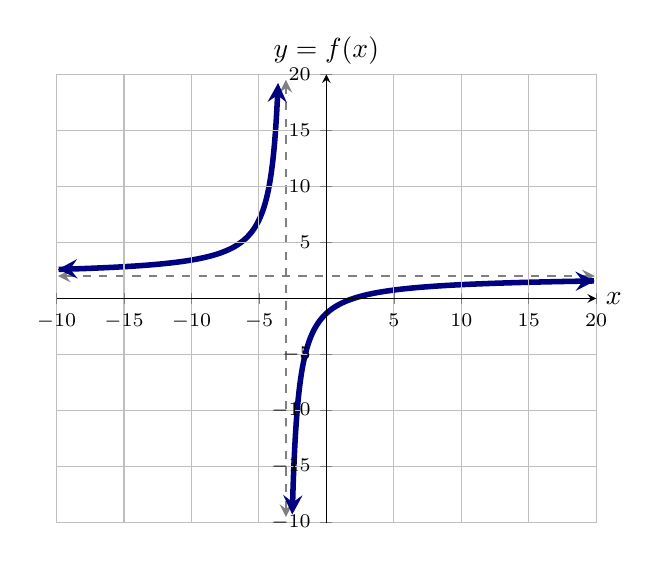
\begin{tikzpicture}
  \begin{axis}[
            domain=-20:20, ymax=20, xmax=20, ymin=-20, xmin=-20,
            axis lines =center, xlabel=$x$, ylabel={$y=f(x)$}, grid = major,
            ytick={-20,-15,-10,-5,5,10,15,20},
            xtick={-20,-15,-10,-5,5,10,15,20},
            yticklabels={$-10$,$-15$,$-10$,$-5$,$5$,$10$,$15$,$20$}, 
            xticklabels={$-10$,$-15$,$-10$,$-5$,$5$,$10$,$15$,$20$},
            ticklabel style={font=\scriptsize},
            every axis y label/.style={at=(current axis.above origin),anchor=south},
            every axis x label/.style={at=(current axis.right of origin),anchor=west},
            axis on top
          ]
          
          \addplot [line width=1, gray, dashed, domain=(-19.5:19.5),<->] ({-3},{x});
          \addplot [line width=1, gray, dashed, domain=(-19.9:19.9),<->] {2};

          \addplot [line width=2, penColor, smooth, samples=300, domain=(-19.9:-3.58),<->] {(2*x-4)/(x+3)};
          \addplot [line width=2, penColor, smooth, samples=300, domain=(-2.53:19.9),<->] {(2*x-4)/(x+3)};


  \end{axis}
\end{tikzpicture}
\end{image}





\[   \lim\limits_{x \to -\infty} f(x)   = 2     \]


\[   \lim\limits_{x \to \infty} f(x)   = 2     \]




\begin{example} Limits 



Let $G(m)$ be defined by the following graph. 

\begin{image}
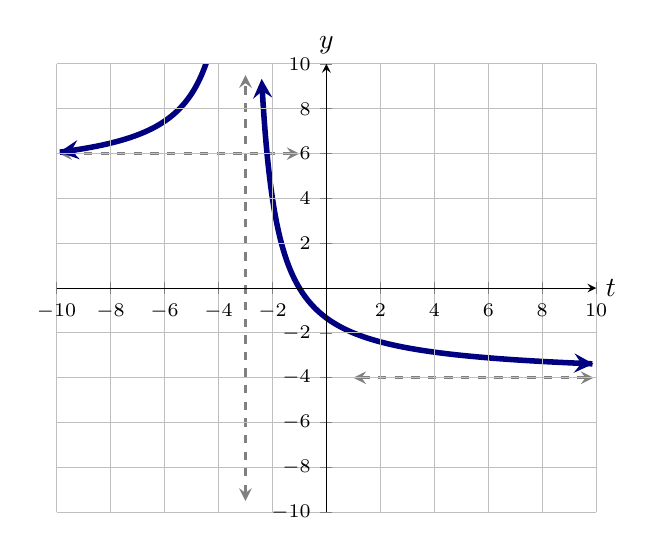
\begin{tikzpicture}
  \begin{axis}[
            domain=-10:10, ymax=10, xmax=10, ymin=-10, xmin=-10,
            axis lines =center, xlabel=$t$, ylabel=$y$, grid = major,
            ytick={-10,-8,-6,-4,-2,2,4,6,8,10},
            xtick={-10,-8,-6,-4,-2,2,4,6,8,10},
            ticklabel style={font=\scriptsize},
            every axis y label/.style={at=(current axis.above origin),anchor=south},
            every axis x label/.style={at=(current axis.right of origin),anchor=west},
            axis on top
          ]
          
          \addplot [line width=1, gray, dashed, domain=(-9.5:9.5),<->] ({-3},{x});
          \addplot [line width=1, gray, dashed, domain=(-9.9:-1),<->] {6};
          \addplot [line width=1, gray, dashed, domain=(1:9.9),<->] {-4};

          \addplot [line width=2, penColor, smooth, samples=300, domain=(-9.9:-3.58),<->] {(6*x-4)/(3*(x+3))+3};
          \addplot [line width=2, penColor, smooth, samples=300, domain=(-2.4:9.9),<->] {(-4*x-4)/(x+3)};


        



           

  \end{axis}
\end{tikzpicture}
\end{image}





\[   \lim_{x \to -\infty} f(x)   = \answer{6}     \]


\[   \lim_{x \to \infty} f(x)   = \answer{-4}     \]



\end{example}

















\begin{example} Limits 



Let $T(y)$ be defined by 



\[
  T(y) = \frac{2 \sin(3y)}{y} \, \text{ defined on } \, (2, \infty)
\]



\begin{image}
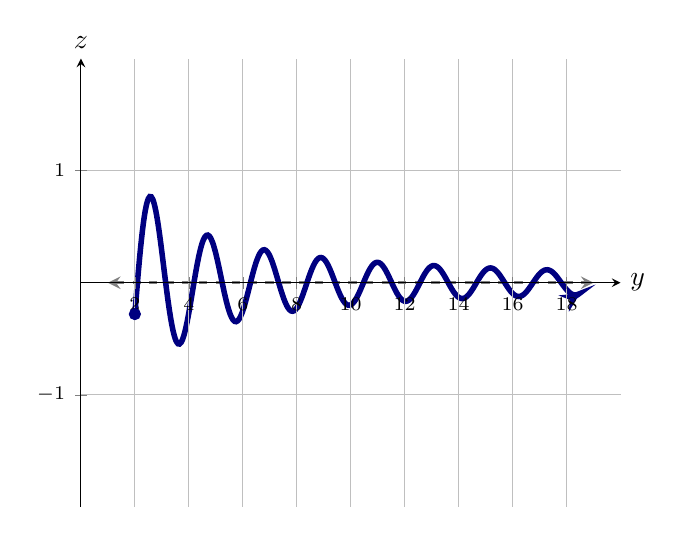
\begin{tikzpicture}
  \begin{axis}[
            domain=0:20, ymax=2, xmax=20, ymin=-2, xmin=0,
            axis lines =center, xlabel=$y$, ylabel=$z$, grid = major,
            ytick={-1,1},
            xtick={2,4,6,8,10,12,14,16,18},
            ticklabel style={font=\scriptsize},
            every axis y label/.style={at=(current axis.above origin),anchor=south},
            every axis x label/.style={at=(current axis.right of origin),anchor=west},
            axis on top
          ]
          
          \addplot [line width=1, gray, dashed, domain=(1:19),<->] {0};

          \addplot [line width=2, penColor, smooth, samples=300, domain=(2:18.5),->] {2*sin(deg(3*x))/x};
          \addplot[color=penColor,only marks,mark=*] coordinates{(2,-0.28)}; 




           

  \end{axis}
\end{tikzpicture}
\end{image}





\[   \lim_{y \to \infty} T(y)   = \answer{0}     \]






\end{example}


















\begin{example} Limits 



Let $R(t)$, with its natural domain, be defined by 



\[
  R(t) = \frac{(2t+5)(t-3)(3t-7)}{(t-8)(t+1)(2t+9)} \,
\]





\[   \lim_{\answer{t} \to \infty} R(t)   = \answer{3}     \]






\end{example}













\begin{center}
\textbf{\textcolor{green!50!black}{ooooo-=-=-=-ooOoo-=-=-=-ooooo}} \\

more examples can be found by following this link\\ \link[More Examples of Function Behavior]{https://ximera.osu.edu/csccmathematics/precalculus/precalculus/functionBehavior/examples/exampleList}

\end{center}





\end{document}
